\subsection{General Considerations}\label{sec:TS_considers}
It is important that individual units of code are manageable and the overall
structure is comprehensible, so that developers and users can navigate the codebase
and determine where new work is to be located.  This simple consideration implies
that \nep\ software should be divided into units that it will be convenient to refer
to as modules, ie.\ sections of code containing everything necessary to perform one
(and only one) aspect of the desired functionality.

The suggested content of a module
describing a single class in the UML sense (see \Sec{TS_lowlevel}, \Tab{TS_umltrans})
implies a minimum of $13$~methods described by separate subroutines/functions,
with examples extending up to $50$, although the latter is there regarded as an excessively large
number of methods.
Many small software libraries also fall into this size range.
Supposing that each subroutine is of a length to fit within one computer window, ie.\
up to about~$60$~lines, the desirable maximum length of a well-designed module file is
$30\times60 = 1\,800$~lines which is a manageable size of file given 
editing software that remembers on restart, the last line accessed (so that it possible
to return immediately to a particular subroutine).
The magnitude of the D3.3 exercise follows from
the fact that comparable software packages probably of somewhat lesser complexity
than \nep\ written in high level languages such as C++ range in size up to~$1\,000\,000$ lines.
Clearly $400$~separate modules is too unwieldy, and there is a need to organise
further into packages which might contain in turn $10$-$50$ modules. 
As a way of providing further indication to developers,
it is helpful to talk of packages as being arranged into layers, as discussed
in ref~\cite[\S\S\,2.4,3.2]{y2re333}, see \Fig{hierarchygroup}.
Then, as prefigured in ref~\cite[Annex~A]{y2re333}, it should be  possible to encapsulate
the necessary complexity in one, albeit large diagram.
\begin{figure}
\centerline{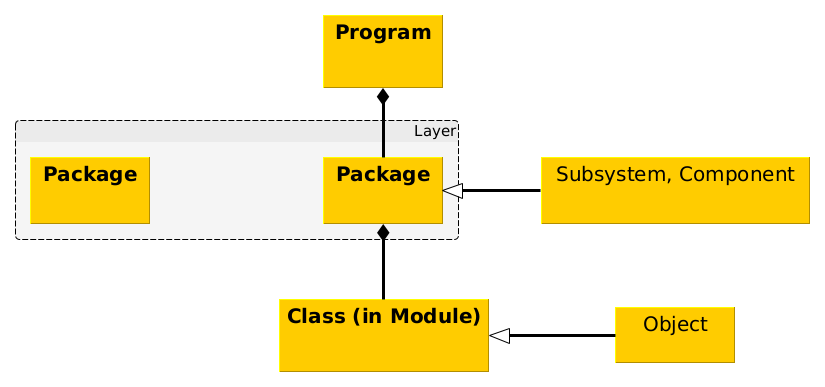
\includegraphics[width=0.7\textwidth]{./png/hierarchygroup.png}}
\caption{
Sketch of relationship between units of large code.
\label{fig:hierarchygroup}}
\end{figure}

\subsection{Considerations for Scientific Software}\label{sec:TS_scistruct}
\subsubsection{Structural Considerations}\label{sec:TS_structure}
In both refs~\cite{y1re331,y2re332}, a figure from Dubey~et~al~\cite{Du16Idea} is reproduced
that illustrates how scientific software may be developed by beginning with an ``infrastructure"
capability into which initially exploratory scientific software is integrated as its worth
is established. Unfortunately for \nep, it is not clear initially what  aspects  of the infrastructure
will be durable and stable, although once the software is more mature, Dubey~et~al's methodology
appears attractive.

The literature referenced in ref~\cite{y2re333}
indicates that scientific software should be produced by aggregation, but is less
helpful as to what is to be aggregated, ie.\  the modular decomposition as to what should
constitute a single module etc.
%Surprisingly little detailed discussion was found in the literature
%after the early book by Booch~\cite{booch}, as to how to create classes in
%the scientific and engineering context, with the exception of Douglass~\cite[\S\,5]{douglass}.
%The ideal would be a way to create classes that enabled rapid development  of code
%that executed efficiently but was easily re-used.
%%where flexibility is also an important consideration,
%Douglass~\cite[\S\,5]{douglass} does not specifically address these last points, but they
%could guide choice of objects in his approach which is reproduced as Appendix~\Sec{TS_objdisc}.

Since the \nep\ development will proceed as a series of \papp s, there is a chance
to refine and redefine an initial modular decomposition with each successive \papp,
recording the results as a UML structure diagram. When generating the corresponding
sequence diagram (ie.\  procedural description), the \papp-based units should be preserved to
facilitate the use of the simpler ones as surrogates for the later more complex \papp s.

To help understand the  aggregation of the software, it should be layered in the obvious manner,
with the higher layers corresponding to greater numbers of aggregated objects. It is also expected
to be useful to classify the modules.
The modules should be arranged into a relatively small number of packages according to, 
eg.\ whether they treat particle generation, matrix coefficient calculation, the main matrix solution, or visualisation.
%\clearpage
\subsubsection{Interactions between Modules}\label{sec:TS_modulint}
Concerning logical interconnections between modules, the 
use of  a directed, acyclic graph~(DAG) structure might be thought mandatory,
particularly to  process the input
data in order to specify coherently the construction of the elements of the solution matrix.
However, as prefigured in ref~\cite{y2re333} for the gyrokinetics code \F{GS2},
the tightly coupled nature of the central edge
physics problem  means that input is more about gathering \emph{all} the data, for only at that point
can fields be computed and only after that may matrix coefficients be computed.

(TODO) ``Information hiding principle" eg.\ input data module ``hides" information about how this is done from
the calculation module: it just passes along parameters in an agreed format.
Can extend this idea on to every level - eg.\ Parnas advocates hiding the hardware from the code -
cf.\  performance portability.
Such modularity  enables work to be efficiently  assigned to a programmer or group.

\subsection{Design of a Module}\label{sec:TS_lowlevel}
\subsubsection{Notation}

%It should be noted that when discussing software in text documents,
%the following conventions in \LaTeX\  are used
%\begin{itemize}
%\item \F{Small capitals} denote a package name
%\item \I{Italics} denote a program name
%\item \T{Fixed width font} denotes any code name or fragment which is not otherwise obviously source code
%\item \B{Bold} denotes a shell script name
%\end{itemize}
%However special fonts are not employed if the class is identified by a
%suitable suffix, thus ``\_m" for a module containing executable code defining methods,
%``\_h" or ``.h" for class attributes (equivalently derived type or namespace code), ``.cpp" for name of file containing 
%C++ source, ``.exe" for an executable, etc.
%Note that Object Fortran has led the way in that 
%requires only one copy of a class's attributes to be compiled, whereas only the very latest versions of C++
%avoid recompilation of namespaces when a .cpp file is changed.
UML nomenclature is preferred herein, for which \Tab{TS_umltrans} provides a limited 
translation into C++ and Object Fortran. % is reproduced as Table~1 in ref~\cite{y2re332}.

\begin{table}[tbph]
\begin{center}
\caption{UML interpreted as Object Fortran and C++ \label{tab:TS_umltrans}}
\begin{tabular}{|p{5cm}|p{5cm}|p{5cm}|}
\hline
UML & Fortran 2003 & C++  \\
\hline
Class & Derived type & Class \\
Part  &  - & Component  \\
Attribute & Component & Data member \\
Method & Type-bound procedure & Virtual Member function \\
Feature  & Component and Type-bound procedure & Data and Virtual Member function \\
Structured class & Extended type & Subclass  \\
Specialisation & Class & Dynamic Polymorphism \\
Generalisation & Generic interface & Function overloading \\
\hline
\end{tabular}
Further insight into UML terminology may be gained from the description
of the patterns in refs~\cite{y2re332,y2re333}.
\end{center}
\end{table}


\subsubsection{Module design}

The focus herein is the structure within a module. Specifically, the module describes a single class or object
(strictly speaking in UML terms, objects are instances of a class), which is
fundamental in that it is defined without use of aggregation.
Tthe software  - consistent with Clerman and Spector~\cite[\S\,11]{clermanspector} -
that is promoted by Arter et al~\cite{fprog} for an object-oriented language, recognises two sizes of fundamental class
and it is easier to start by considering the smaller, denoted smallobj\_m.

Module smallobj\_m does not have a separate attributes file, but will typically still use or access
three or more yet more fundamental classes, namely
\begin{itemize}
\item log\_m for logging errors or warnings in code execution, and checkpointing values of selected variables
\item const\_numphys\_h for numerical values of important mathematical and physical constants relevant to plasma physics
\item const\_kind\_m to specify precision of representation of real and integer values, together 
with formatting to be used for their output (in fact contains no executable code)
\item date\_time\_m to return the date and time in either a verbose or minimal format
\item misc\_m to form miscellaneous operations found to be common to many modules
\end{itemize}
In outline, the  methods or operations associated with \T{smallobj} allow data to be read from a named file,
used in the construction of an object, and output to disc file. The file is given a numeric identifier~\T{ninso}
(file~unit) when it is opened. Data used to construct the  object forms a single \T{namelist} block, viz.\ 
a list of arbitrary code variables that may (or not) be assigned values in the input file using a attribute-value notation.
Namelist variables should have long names that promote a good user interface, and
be given default values in case they are not input.
The style encourages checking that inputs have acceptable values, for example lie in expected ranges,
but there is no equivalent of eg.\ the Cerberus Python data validation package~\cite{cerberuswebsite},
users must explicitly code checks and calls
to log\_m if the values are questionable or erroneous. (It is hoped that this can be automated based
on a \LaTeX \ table describing input symbols. After successful checks, the values in
the namelist are copied into the data type sonumerics\_t, whence it is supposed that a single subroutine then
instantiates the smallobj\_t object. Another routine performs
output of this object, either to a directly specified file unit, or
to the standard output by default, in the simple text format of a variable name followed by its value on the following
line. As might be expected, there are also routines to `delete' the object, ie.\ to deallocate
any constituent arrays, and to close the input file.
The precise list of member functions (or methods in the UML nomenclature) is
\begin{itemize}
\item initfile,  open input file
\item readcon,  read data from input file
\item generic,  generic subroutine to instantiate object
\item write, write out object to standard output, or to file opened by another object
\item delete, delete object
\item close, close input file
\end{itemize}

Module bigobj\_m has a separate file for its attributes (\emph{aka} namespace), which it will
normally still use or access
like the yet more fundamental objects listed for smallobj\_m. However the data types
defined in bigobj\_h are of the same kind as those in smallobj\_m, viz.\ bonumerics\_t
to hold input data which is used to define bigobj\_t by calling the \T{solve} subroutine
(rather than the subroutine \T{generic} in the case of smallobj\_m). Apart from
this last  exception, the methods in bigobj\_m are a superset of those in smallobj\_m.
The additional methods recognise that instantiation may involve
more than one routine and in particular may involve use of a specially defined
function \T{fn}, demonstrating the STRATEGY Pattern or possibly TEMPLATE Pattern.
This function may be determined by a formula identified in the input,
giving  the option for a developer or determined user of adding their own code to define
a new function. The range of allowable outputs is much extended. Thus there
is a separate routine provided for output to the log file using what will
probably be a lengthy list of calls to log\_value\_m. More likely to be useful  is a routine
to open an .out file on a file unit given the number~\T{noutbo} on opening, which
becomes the default unit for writing out the object in \T{bigobj\_write}.
There are also provided separate skeleton routines intended to provide output
in a format suitable respectively for visualisation by \F{gnuplot} and \F{ParaView},
and of course routines to close files and delete the object.
The precise list of member functions for bigobj\_m is as follows
where those also found in smallobj\_m are enclosed in parenthesis:
\begin{itemize}
\item (initfile),  open input file
\item (readcon),  read data from input file
\item solve,  generic subroutine to manage instantiation of object
\item userdefined,  user-defined method or function
\item fn, general external function call
\item dia, write object diagnostics to log file
\item initwrite, open new file, making up name which defaults to having .out suffix
\item (write), write out object to standard output, or to file opened by \T{bigobj}
\item writeg, write out object suitable for  visualisation by \F{gnuplot}
\item writev, write out object suitable for  visualisation by \F{ParaView} 
\item (delete), delete object
\item (close), close input file
\item closewrite,  close write file opened by \T{initwrite}
\end{itemize}

Thus the skeleton object is defined by a formula plus data input from disc,
and since both are saved internally as features, the instantiation may be deferred as necessary,
so-called `lazy initialisation'.
It will be noticed that other variables in bigobj\_m such as unit number are hidden, ie.\ cannot be accessed by
other modules. In fact a common addition to the default modules is a method function \T{getunit} that returns \T{ninbo},
illustrating the approved way of accessing such data.

%The source as mentioned in ref~\cite{y2re333} may be obtained by download of
%program~\I{smardda-qprog}~\cite{qprogwebsite}.
The reason for the emphasis on input and output from and to disc (I/O)
is to facilitate the construction of a test harness
for an objects in the style of bigobj\_m, and indeed the aggregations of such objects.  
The use of ``attribute-value" in I/O gives flexibility to the developer, since new variables may be
added without the need to modify existing input files or output processing. Output processing is further
discussed in \Sec{TS_procio}.

%In the course of a software development, the source code relating to an object naturally grows
%with the addition of further subroutines in the module file.
%Since \nep\ is anyway going to have to describe the equilibrium magnetic field~${\mathbf B}$ it
%is worth examining what such growth led to the beq\_m \F{SMARDDA} module
%besides the standard routines listed above.
%In fact beq\_m grew to $50$~routines (the number probably indicating a need for refactoring) so they will
%not be listed in full. $13$ of the new routines are concerned with either reading or writing from disc,
%reflecting the ability to handle a range of formats of the so-called `eqdsk'~type, plus an ability
%to define the magnetic field analytically. The eqdsk and analytic description assume axisymmetry
%with the field defined by the magnetic flux function~$\psi(R,Z)$ where $(R,Z)$ are cylindrical polar coordinates
%centred on device major axis. Much of the module complexity is accounted for by the needs either to verify
%that the field has been correctly read in as the `eqdsk' format is not standardised, or
%to return ${\mathbf B}$ in either flux, polar or Cartesian coordinates,  in formats avoiding storage on
%a whole~$360^o$ mesh. Onto this structure
%was subsequently bolted capabilities to superimpose a non-axisymmetric vacuum field (which is not strictly an
%equilibrium field) and to track through the $\psi$-landscape for various purposes.
%
%Representative routines in beq\_m are
%\begin{itemize}
%\item fixorigin, which fixes a problem encountered when the data in
%the eqdsk extends to $R=0$ because eg.\ the $Z-$component of ${\mathbf B}$ is defined as $(1/R) \partial\psi/ \partial R$.
%\item sense, which returns the sense of helicity of the field
%\item psilt, to calculate the actual range of values of $\psi$ by resolving possibly conflicting inputs
%\item ctrackc, return the track in~$(R,Z)$ running through the plasma centre of the extremum of $\psi$
%\item init, which initialises the field, the equivalent of \I{solve} and/or \I{generic}
%\end{itemize}
%Arguably $\psi$ should be disaggregated as a separate class for the purposes
%of tracking extrema etc. In one sense, it is already separate because  it constitutes a
%2-D spline class, being of type spl2d\_t defined in modules spl2\_m. 
%However the latter is conceptually a mathematical construct, whereas the analyses in beq\_m are
%physically conceived, which is why they were placed there. This illustrates one of the difficult dilemmas
%that may arise from the object-oriented approach in scientific applications. Another feature
%of scientific work is the use of simple analytic formulae either for testing purposes 
%or to include an effect such as field ripple to get a qualitative feel for its influence,
%rather than always using detailed machine data to get a full quantitative evaluation.


\subsection{Processing Module Output}\label{sec:TS_procio}
The number of I/O subroutines can be criticised.
For many testing purposes an interactive debugger is adequate,
and for most others that one output file is sufficient provided it is in a attribute-value
format such as JavaScript Object Notation~(JSON) or in a self-documenting format such as the 
Network Common Data Form~(netCDF), to be interpreted by any suitable visualisation software.

The problem with scientific software, worse
at Exascale, is the volume of data to be handled so that the ability to visualise large arrays
as well as large numbers of small arrays is essential (no debugger as far as is known has 
such a visualisation feature).  Moreover, the actionable aspect of \nep\ further means
that any postprocessing of a generic file must also be carefully performed. Thus while
a generic output file could be processed by say Linux \T{awk} script into a form suitable for
\F{gnuplot} processing, this gives rise to a need for providing documentation and
provenance for the script, which is at minimum a nuisance. Worse is the risk that the amount of
data to be processed may be so large as to lead to significant
delay and maybe even system or other issues not handled well if at all by the script, all of which
may be extremely time-consuming to resolve. Other conversion software may not be available
or properly implemented on the target machine.
Thus even for debugging purposes, it seems desirable that as much as possible of the processing
is done within the main code, and for production runs, output in a format
directly readable by say~\F{ParaView} should also speed the post-processing.
Since netCDF may be read directly by~\F{ParaView}, this is recommended.


